\chapter {Testing \& Results of Support Vector Classification}

\section{Classification of Testing Data}
To determine optimal performance, the system was setup with different numbers of training points. A variable number of parameters were used to test the improvement in performance of the SVM classification. The testing data was gathered by hand, and later automated for ease of testing. After gathering the points, they were classified into their respective categories with a premade mask described earlier. The final accuracy was measured as a percentage of correctly classified points for the total image, and of points that were close to the optimal hyperplane.
\section{Overall Effect}
The main parameters used in the SVM are:\\ 
\\
\textbf{XY (Pixel Location)}\\
\textbf{L*a*b* Pixel value} \\
\textbf{L*a*b* Radial Blur} \\
\textbf{L*a*b* Sobel} \\
\\
To evaluate the parameters in effectiveness their accuracies are compared individually. In figure \ref{fig:15_gaussianlabtrainingonly} the images were gained by passing each point through the SVM, and returning a green pixel if the point was classified as a door otherwise a red pixel would be returned. The accuracies presented are from testing 33\% of the total sample points used with predefined classification -- where 66\% are used for training the SVM.
\newpage


\begin{figure}[h]
        \centering
        \begin{subfigure}[b]{0.3\textwidth}
                \centering
                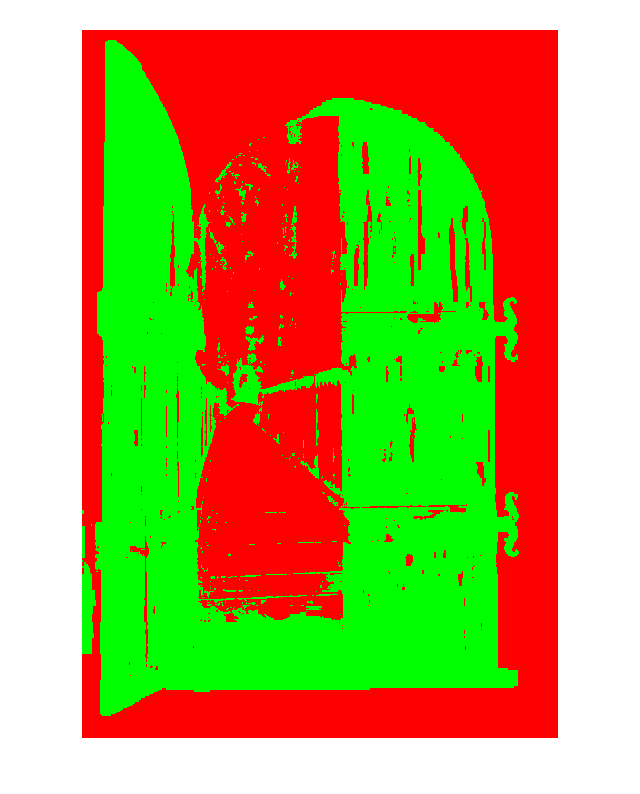
\includegraphics[width=1.6in]{14_labtrainingonly}
                \caption{L*a*b* Pixel data -- 89.87\% accuracy \\*}
                \label{fig:14_labtrainingonly}
        \end{subfigure}%
        ~ %add desired spacing between images, e. g. ~, \quad, \qquad etc.
          %(or a blank line to force the subfigure onto a new line)
        \begin{subfigure}[b]{0.3\textwidth}
                \centering

                
\includegraphics[width=1.6in]{15_gaussianlabtrainingonly}
                \caption{Gaussian Radial Blur (L*a*b* pixel data) -- 90.16\% accuracy}
                \label{fig:15_gaussianlabtrainingonly}     
        \end{subfigure}
        ~ %add desired spacing between images, e. g. ~, \quad, \qquad etc.
          %(or a blank line to force the subfigure onto a new line)
        \begin{subfigure}[b]{0.3\textwidth}
                \centering

                
\includegraphics[width=1.6in]{13_xytrainingonly}
                \caption{XY Pixel Location -- 82.53\% accuracy \\*}
                \label{fig:13_xytrainingonly}
        \end{subfigure}
         \begin{subfigure}[b]{0.3\textwidth}
                \centering

                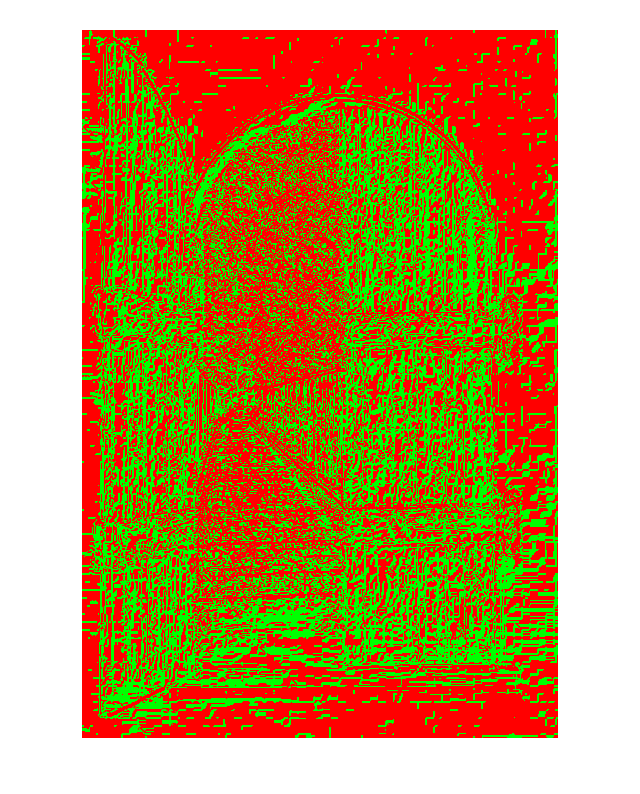
\includegraphics[width=1.6in]{16_sobeltrainingonly}
                \caption{Sobel information -- 61.82\% accuracy \\*}
                \label{fig:16_sobeltrainingonly}
        \end{subfigure}
        \begin{subfigure}[b]{0.3\textwidth}
                \centering

                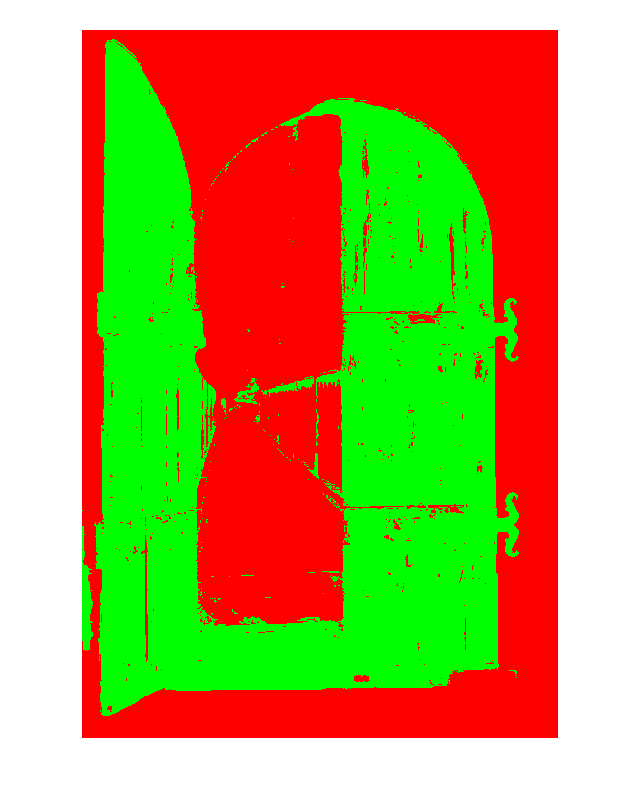
\includegraphics[width=1.6in]{17_labsobelgaussiantraining_93}
                \caption{L*a*b*, Gaussian Radial Blur, and Sobel -- 92.22\% accuracy}
                \label{fig:17_labsobelgaussiantraining_93}
        \end{subfigure}
        \begin{subfigure}[b]{0.3\textwidth}
                \centering

                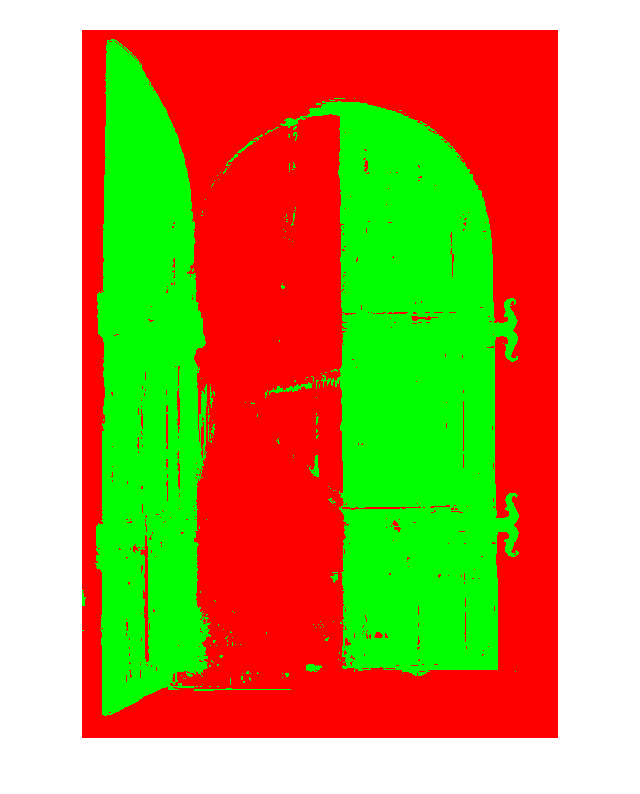
\includegraphics[width=1.6in]{18_labsobelgaussianxytraining_96}
                \caption{XY, L*a*b*, Gaussian Radial Blur, and Sobel -- 94.71\% accuracy}
                \label{fig:18_labsobelgaussianxytraining_96}
        \end{subfigure}

        \caption{Results of Differing SVM information, individual testing -- using 2000 sample points. Accuracy values are from edge case testing, total value is higher}\label{fig:labResults}
\end{figure}
As seen in figure \ref{fig:labResults}, it was determined that the inputs that yielded the most optimal results were the XY position, L*a*b* colour data, the Sobel filter data, and the Gaussian Radial Blur. In effect, the pixel position and the pixel colour alongside with the derivation and the integration of the pixel L* data. These have shown to be effective parameters for classification. The hardest parts for the SVM to properly classify were areas with both similar colour and texture to the door. In these areas, the SVM had a higher probability to return false positive results.

\section{Outcome}

By limiting the number of training points for the support vector machine, it was possible to achieve performances of 90\% and above. But the position of these points had a greater effect on the results than when the number of points was higher. As expected, the results were very sensitive to the position of the training points; more points will cause the support vectors to be further away from the optimal hyperplane. Thus, the variance in the accuracy with differing test sets decreased when the total number of points increased. This effect can be seen in figure \ref{fig:12_testsizevsaccuracy}.

\begin{figure}[ht]
    \centering
    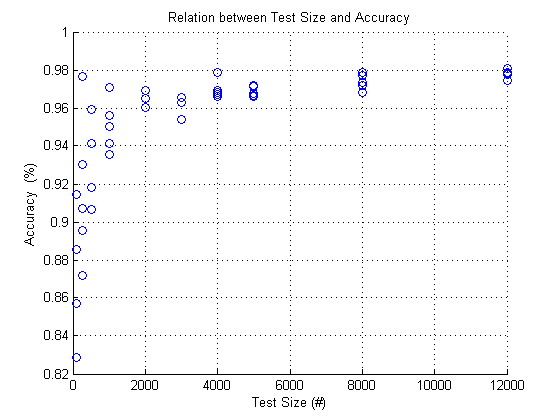
\includegraphics[height=3in]{12_testsizevsaccuracy}
    \caption{Changes in accuracy in the SVM from variance in the training set size.}
    \label{fig:12_testsizevsaccuracy}
\end{figure}

Using X and Y as the additional input information was good at a higher number of training points, but did not show as good of a performance as the only parameter, or when using smaller training sets. The L*a*b* Gaussian Radial blur information was by far the best for contributing to overall accuracy. 

\begin{figure}[h]
        \centering
        \begin{subfigure}[b]{0.2\textwidth}
                \centering
                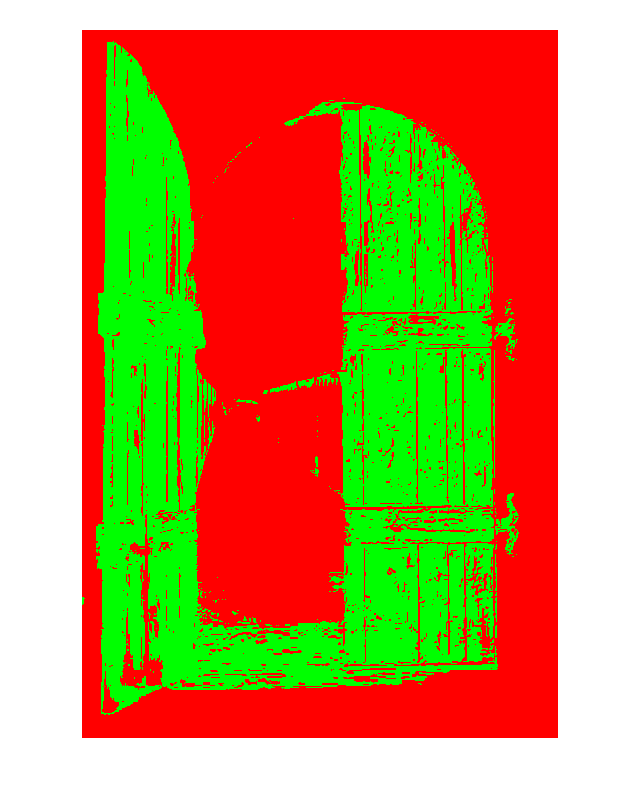
\includegraphics[width=1.6in]{19_labsobelgaussianxytraining_90-3275_80_100}
                \caption{100}
                \label{fig:19_labsobelgaussianxytraining_90.3275_80_100}
        \end{subfigure}%
        ~ %add desired spacing between images, e. g. ~, \quad, \qquad etc.
          %(or a blank line to force the subfigure onto a new line)
        \begin{subfigure}[b]{0.2\textwidth}
                \centering

                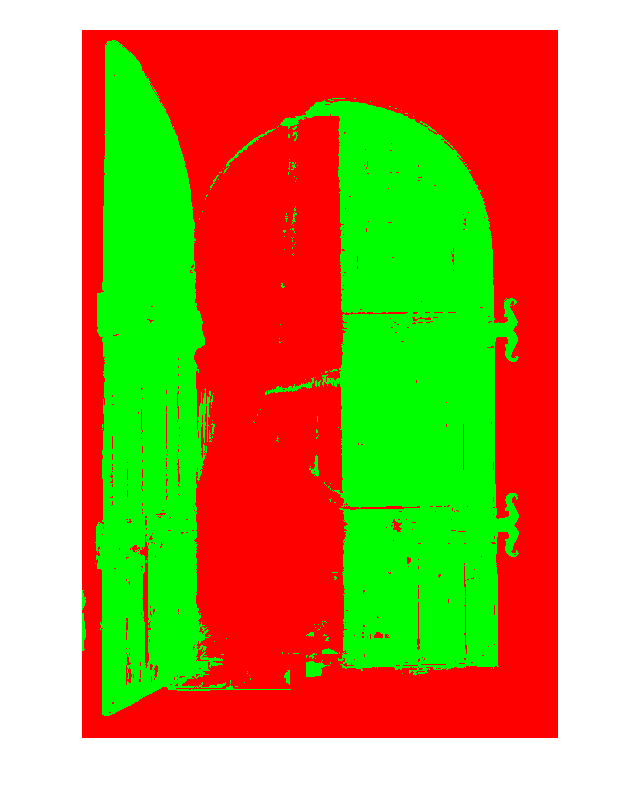
\includegraphics[width=1.6in]{22_labsobelgaussianxyexample_97-5312_96-0823_3000}
                \caption{3000}
                \label{fig:22_labsobelgaussianxyexample_97.5312_96.0823_3000}     
        \end{subfigure}
        ~
        \begin{subfigure}[b]{0.2\textwidth}
                \centering

                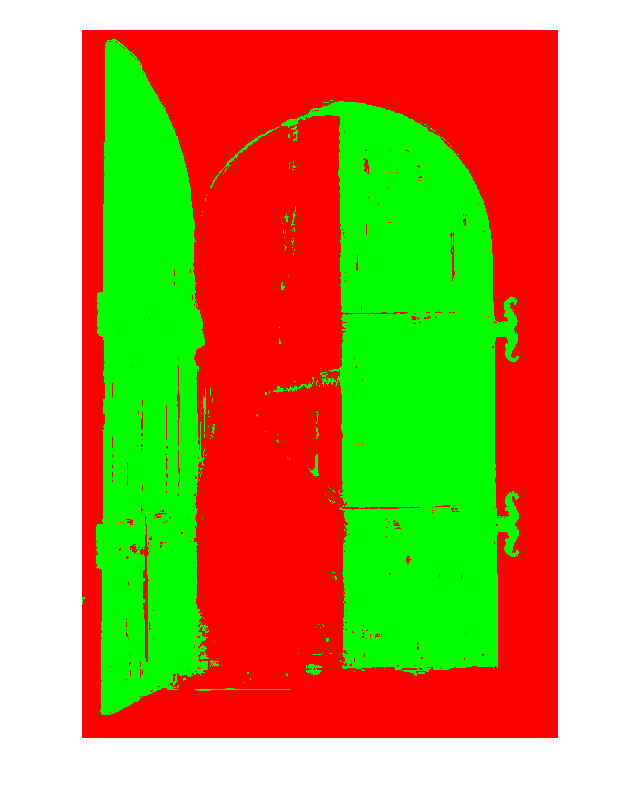
\includegraphics[width=1.6in]{21_labsobelgaussianxyexample_98-1101_96-7173_6000}
                \caption{6000}
                \label{fig:21_labsobelgaussianxyexample_98.1101_96.7173_6000}     
        \end{subfigure}
        \begin{subfigure}[b]{0.2\textwidth}
                \centering

                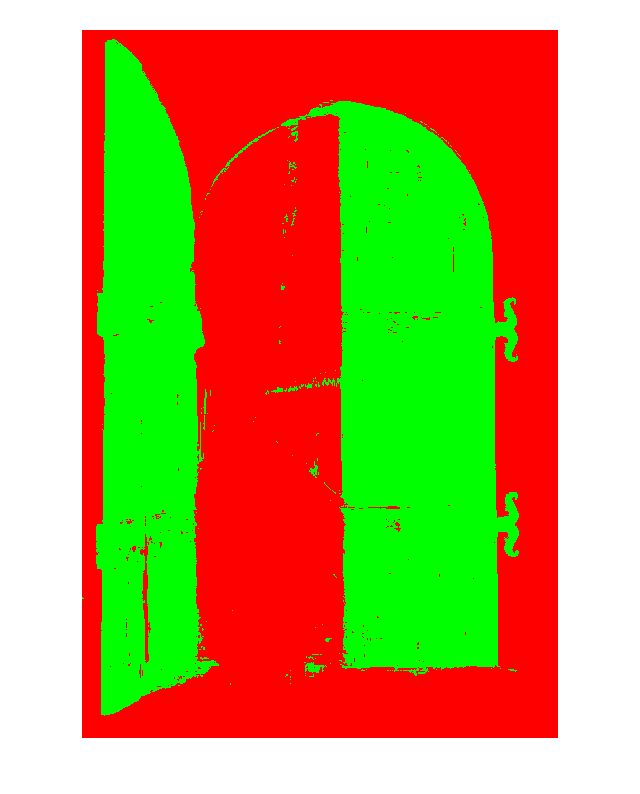
\includegraphics[width=1.6in]{20_labsobelgaussianxyexample_98-5724_97-4761_12000}
                \caption{12000}
                \label{fig:20_labsobelgaussianxyexample_98.5724_97.4761_12000}     
        \end{subfigure}
        \caption{Results of Differing sample points}\label{fig:samplepoints}
\end{figure}

\begin{center}
  \begin{tabular}{| c | c | c | c | }
    \hline
    \textbf{Total Points} & \textbf{Training Set size} & \textbf{Testing set accuracy} & \textbf{Overall accuracy} \\ \hline
    100 & 66 & 80\% & 90.33\% \\ \hline
    3000 & 1980 & 96.08\% & 97.53\% \\ \hline
    6000 & 3960 & 96.72\% & 98.11\% \\ \hline
    12000 & 7920 & 97.48\% & 98.57\% \\ 
    \hline
  \end{tabular}
\end{center}

As seen in figure \ref{fig:samplepoints} there are diminishing returns when increasing the number of points that are used to train the SVM. While it is possible to get good results at low number of sample points, the performance depends far more on the position of the points.